\documentclass[unicode,10pt]{beamer}
\usetheme{ttiposter}

\usepackage{luatexja}
\usepackage{luatexja-fontspec}
\usepackage{geometry}
\usepackage{graphicx}
\usepackage{multicol}
\usepackage{subcaption}
\captionsetup{compatibility=false}

\setmainjfont{ipagp.otf}
\beamertemplatenavigationsymbolsempty

\geometry{a4paper,portrait,left=2truemm,width=206truemm,right=2truemm}
\newlength{\mycolumnwidth}
\setlength{\mycolumnwidth}{0.495\textwidth}

\newcommand{\arrow}{\textcolor{ttiblue}{\textbf{→}}\hspace{1ex}}
\newcommand{\itemtitle}[1]{\textbf{#1}\\}
\newcommand{\fire}[1]{\textcolor{red}{\textbf{#1}}}
\newcommand{\doublecolumns}[4]{
    \begin{minipage}[t]{#1}
      #2
    \end{minipage}
    \begin{minipage}[t]{#3}
      #4
    \end{minipage}}


\title{文書・文間及びカテゴリ間の関係を考慮したレーティング予測}
\institute{知能数理研究室}
\author{12056 外山 洋太}
\date{\today}



\begin{document}
\begin{frame}[t]
\vspace{-1em} % HACK

\begin{columns}[onlytextwidth,t]
  \begin{column}{1.1\mycolumnwidth}
    \begin{block}{背景と目的}
      \begin{itemize}
        \item 対象問題:多カテゴリにおける商品レビューのレーティング予測
        \item 研究意義:企業における文書からの商品の評判分析
        \item 目的:\fire{文書・文間の関係}及び\fire{カテゴリ間の関係}を
                    考慮した\\レーティング予測の実現
      \end{itemize}
    \end{block}
  \end{column}
  \begin{column}{0.9\mycolumnwidth}
    \begin{figure}
      \hspace*{\fill} % HACK
      \begin{subfigure}[t]{0.4\linewidth}
        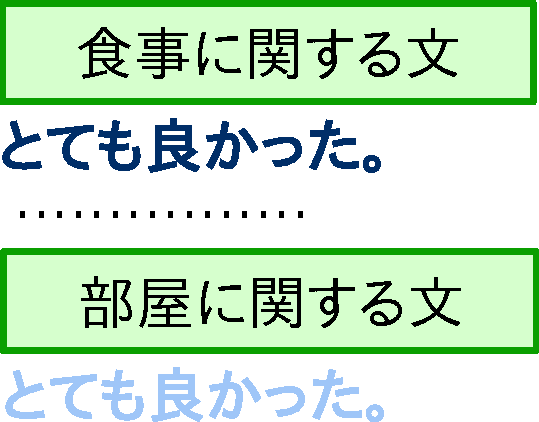
\includegraphics[width=0.9\linewidth]
                        {fig/global_relations_among_sentences_v2.pdf}
        \subcaption*{文章・文間の関係}
      \end{subfigure}
      \hfill % HACK
      \begin{subfigure}[t]{0.5\linewidth}
        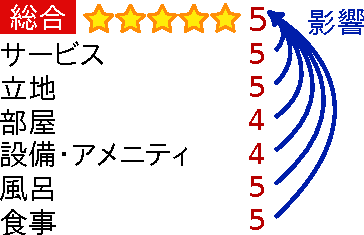
\includegraphics[width=0.9\linewidth]
                        {fig/relations_among_rating_categories.pdf}
        \subcaption*{カテゴリ間の関係}
      \end{subfigure}
      \hspace*{\fill} % HACK
    \end{figure}
    \vspace{0.5em}
    %\begin{figure}
    %  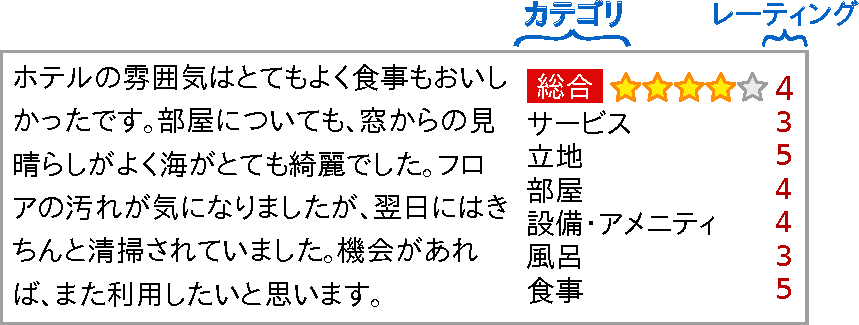
\includegraphics[width=0.9\linewidth]{fig/review.pdf}
    %  \caption{複数のカテゴリを持つ商品レビューの例}
    %\end{figure}
  \end{column}
\end{columns}

\begin{block}{関連研究}
  \begin{columns}[onlytextwidth,t]
    \begin{column}{0.3\textwidth}
      \begin{itemize}
        \item \itemtitle{隠れ状態を用いたホテル\\レビューのレーティング予測
                         \cite{fujitani15}}
          \begin{itemize}
            %\item 複数カテゴリでの予測に対応
            \item 文毎のレーティングからレビュー全体のレーティングを予測
            \item カテゴリ間の繋がりを\fire{手調整によって変化}させ考慮
          \end{itemize}
        %\item \itemtitle{ニューラルネットワーク}
        %  \begin{itemize}
        %    \item 神経回路を模した機械学習手法
        %    %\item 分類問題に適用可能
        %    %\item 文書・文間やカテゴリ間の複雑な関係を考慮
        %  \end{itemize}
      \end{itemize}
      %\begin{figure}
      %  \includegraphics[width=0.7\linewidth]
      %      {fig/fujitani_miml_relations_among_rating_categories.pdf}
      %\end{figure}
    \end{column}

    \begin{column}{0.375\textwidth}
      %\begin{itemize}
      %  \item \itemtitle{パラグラフベクトルの目的関数:$L$}
      %    \doublecolumns{0.575\linewidth}{
      %      \vspace{-1.5em} % HACK
      %      \begin{gather*}
      %        L = \frac{1}{T} \sum^{T}_{t = k}
      %            \log p(w_t | w_{t-k}, ..., w_{t-1}),
      %          \label{eq:ParagraphVector} \\
      %        p(w_t | w_{t-k}, ..., w_{t-1})
      %          = \frac{e^{y_{w_t}}}{\sum_i e^{y_i}},
      %          \nonumber \\
      %        y = b + Uh(w_{t-k}, ..., w_{t-1}, d; W, D) \nonumber
      %      \end{gather*}
      %    }{0.4\linewidth}{
      %      $d$:文章 \\
      %      $w_i$:単語 \\
      %      $W$:単語行列 \\
      %      $D$:文章行列 \\
      %      $k$:ウィンドウサイズ \\
      %      $T$:文章の単語数 \\
      %      $U$:射影行列 \\
      %      %ある単語の周辺を表す区間をウィンドウという。
      %      %$p$はsoftmax関数により正規化された、
      %      %文脈から現在の単語が導かれることの尤度
      %      %$p$を構成する$y$は現在の単語とウィンドウ内の
      %      %単語及び現在の文章から導出
      %      $h$:ベクトルを結合する関数
      %    }
      %\end{itemize}
      \begin{itemize}
        \item \itemtitle{パラグラフベクトル\cite{quoc14}}
          \begin{itemize}
            \item 文や文書を、その意味を表す実数ベクトルに変換
            \item \fire{レーティング予測において優れた性能}
            \item 右図の例:単語「肉」を予測するように「おいしい」と「魚」、
                  「と」のベクトルを学習
          \end{itemize}
      \end{itemize}
    \end{column}

    \begin{column}{0.325\textwidth}
      \begin{figure}
        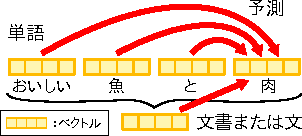
\includegraphics[width=0.9\linewidth]{fig/paragraph_vector_v2.pdf}
        \caption*{パラグラフベクトルの学習}
      \end{figure}
    \end{column}
  \end{columns}
\end{block}

\begin{block}{提案手法}
  \begin{columns}[onlytextwidth,t]
    \begin{column}{\mycolumnwidth}
      %\begin{itemize}
      %  \item \itemtitle{特徴}
        %\item \itemtitle{レーティング予測の流れ}
        %  \begin{enumerate}
        %    \item パラグラフベクトルによってレビュー内の \\
        %          文書全体及び各文の意味表現を生成
        %    \item 文ベクトルをレビュー毎に重み付け平均 \\
        %          \arrow 全てのレビューで文の数を統一
        %    \item ニューラルネットワークで多ラベル多クラス分類
        %  \end{enumerate}
      %\end{itemize}
      %\begin{flalign*}
      %  \begin{cases}
      %    \text{入力:レビューの文書} \\
      %    \text{出力:カテゴリ毎のレーティング}
      %  \end{cases} &&
      %\end{flalign*}
      \begin{itemize}
        \item 文書・文間及びカテゴリ間の関係を考慮したレーティング予測
      \end{itemize}
      \begin{figure}
        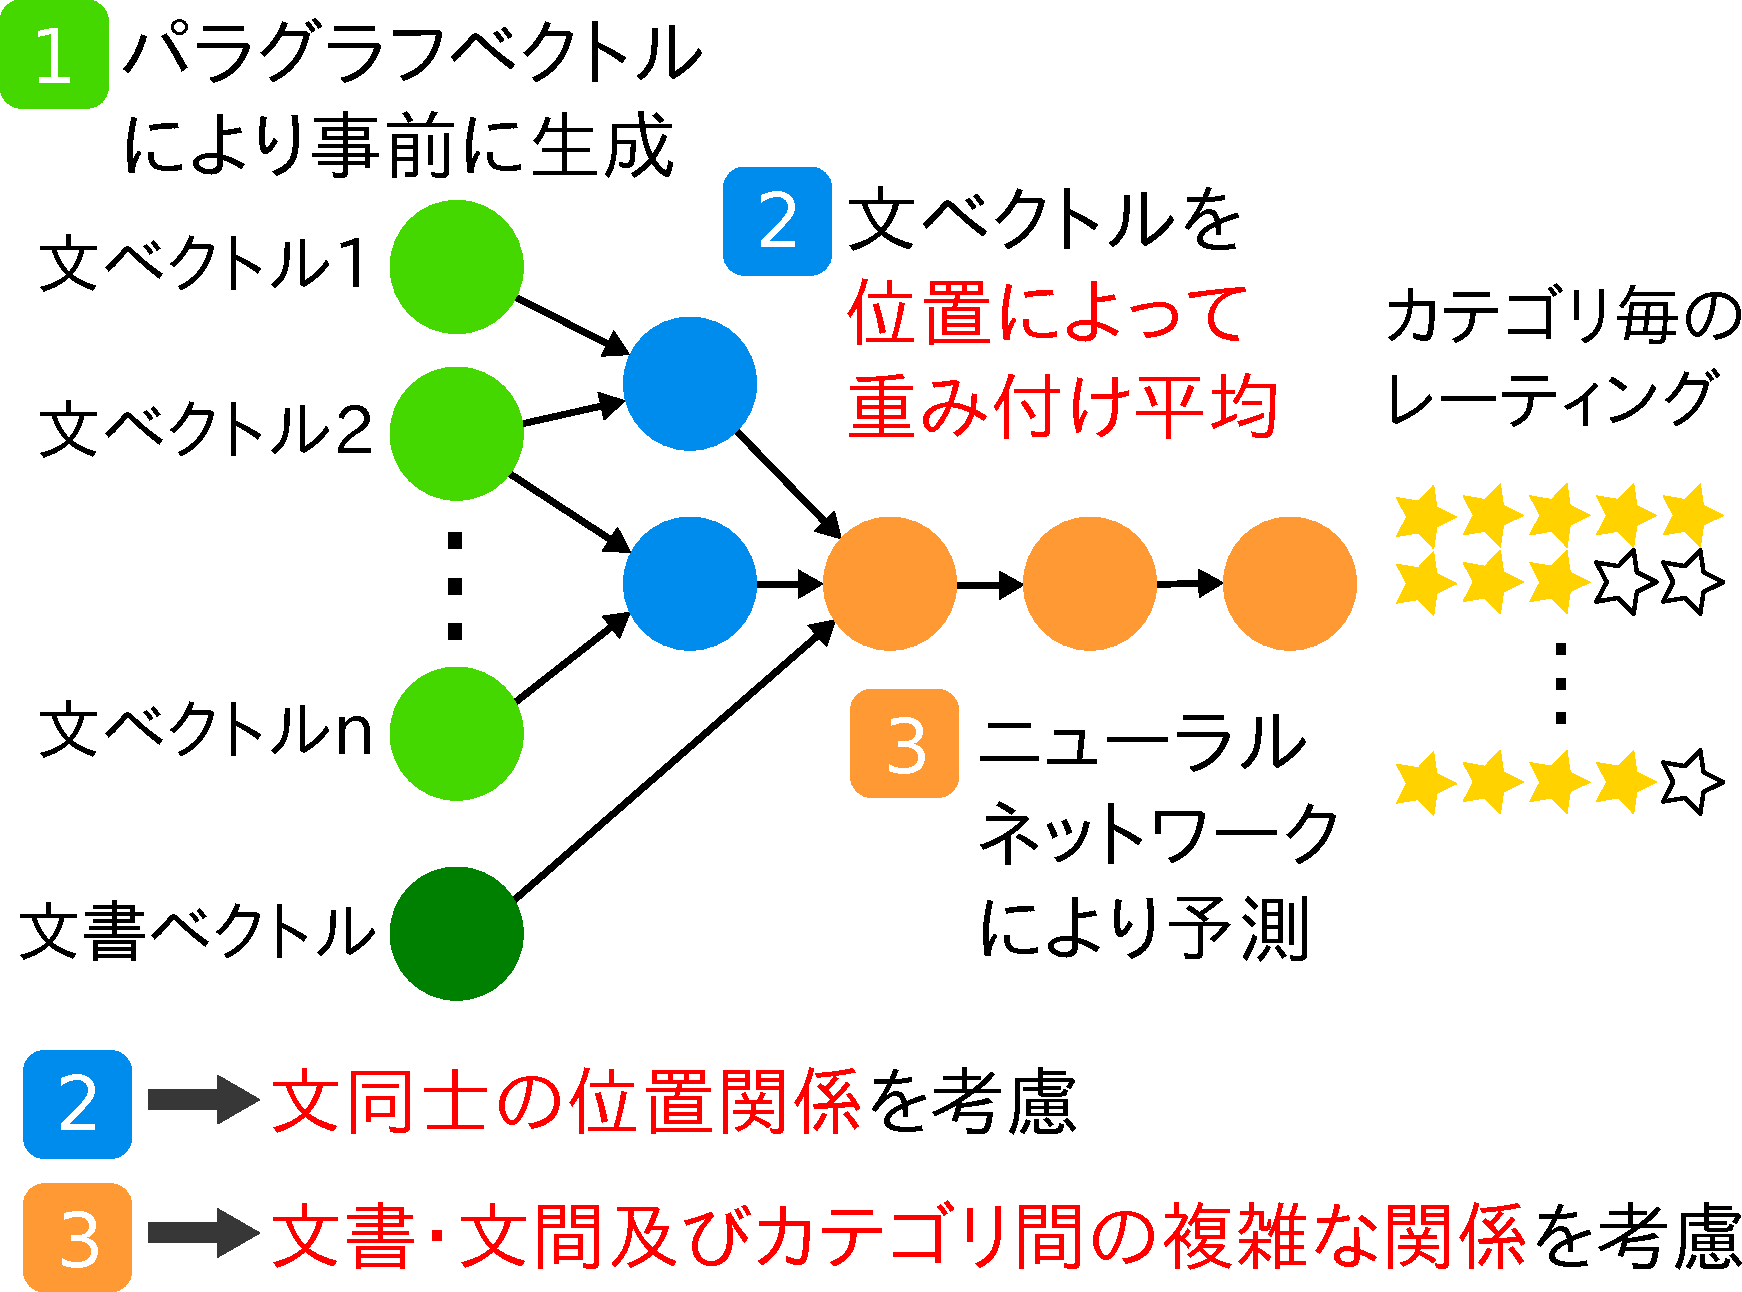
\includegraphics[width=0.9\linewidth]
                        {fig/model_with_much_detailed_processes.pdf}
        \caption*{提案手法における予測モデル}
      \end{figure}
      %\begin{itemize}
      %  \item (2) \arrow \fire{文同士の位置関係}を考慮
      %  \item (3) \arrow \fire{文書・文間及びカテゴリ間の関係}を考慮
      %\end{itemize}
    \end{column}

    \begin{column}{\mycolumnwidth}
      \begin{itemize}
        \item \itemtitle{文ベクトルを位置によって重み付け平均}
          \begin{figure}
            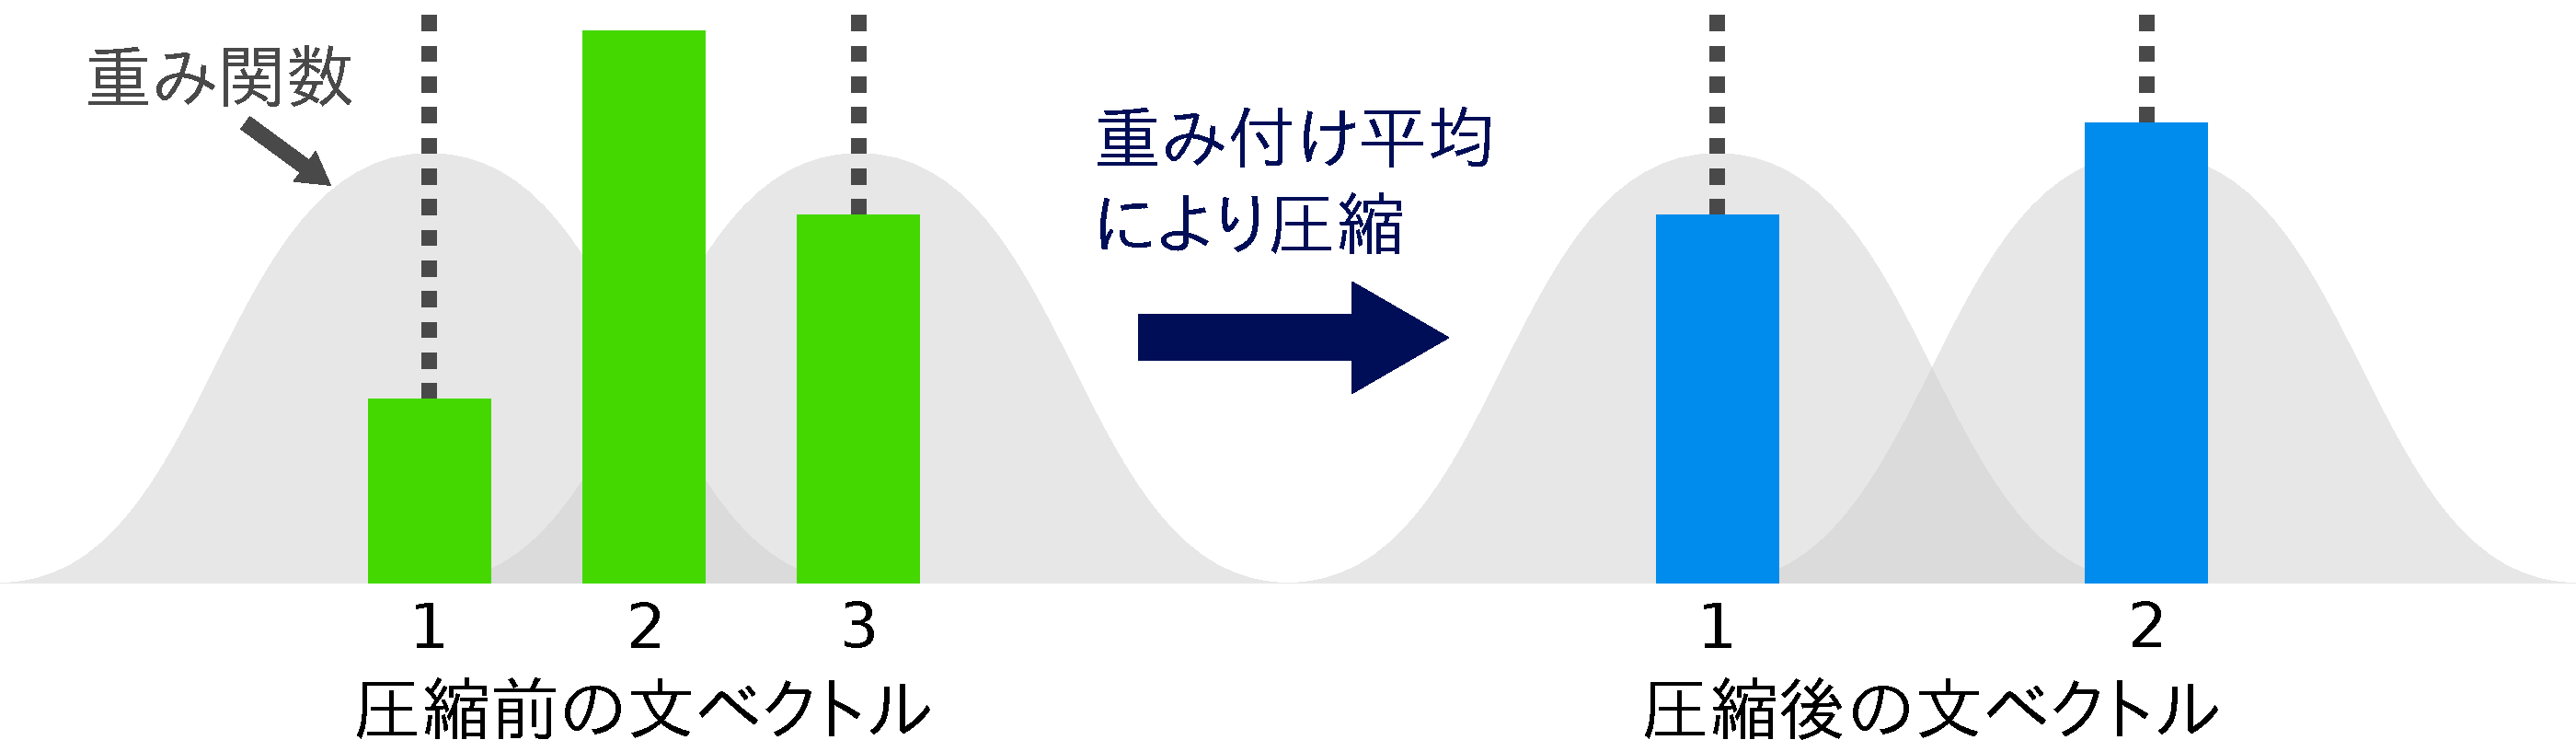
\includegraphics[width=\linewidth]
                            {fig/what_are_you_weighting_for.pdf}
          \end{figure}
          %\doublecolumns{0.625\linewidth}{
          %  \abovedisplayskip=0pt
          %  \begin{gather*}
          %    \mathbf{t}_{i_{part}} = \sum_{i_{sent}}
          %                            \frac{w(x_{i_{part}}(i_{sent}))}
          %                                 {|\sum_{i_{sent}'}
          %                            w(x_{i_{part}}(i_{sent}'))|}
          %                            \mathbf{s}_{i_{sent}},
          %    \label{eq:WeightedAverageSV} \\
          %    x_{i_{part}}(i_{sent}) = \frac{i_{sent} - i_{part}}{\#partitions},
          %    \nonumber \\
          %    w(x) = \begin{cases}
          %      \frac{1}{2} (\cos(\pi|x|) + 1) &\text{if $|x| <= 1$} \\
          %      0 &\text{otherwise}
          %    \end{cases} \nonumber
          %  \end{gather*}
          %}{0.35\linewidth}{
          %  \small
          %  $i_{sent}$:レビュー内の文のインデックス \\
          %  $\#partitions$:重み付け平均後の文ベクトルの数\\
          %  $i_{part}$:重み付け平均後の文ベクトルのインデックス\\
          %  $\mathbf{s}_{i_{sent}}$:文ベクトル
          %  %\footnote{重み付けの関数には$\cos$関数の他に、
          %  %$x$に対して線形に重みを減少させるような関数や、
          %  %単純に文を区画毎に平均するような関数も考えられる。
          %  %区画毎に平均する関数は他の2つより正答率が低く、線形な関数と
          %  %$\cos$関数はほぼ同じ正答率を示したため、$\cos$関数を採用した。}
          %}
        \item \itemtitle{ニューラルネットワークの目的関数:$E$}
          \doublecolumns{0.6\linewidth}{
            \begin{gather*}
              E = - \sum^{N}_{n = 1} \sum^{C}_{c = 1} \sum^{K}_{k = 1}
                    d_{nck} \log{y_{ck}(x_n; w)},
              \label{eq:NNObjective} \\
              y_{ck}(x_n; w) = \frac{e^{u_{ck}(x_n; w)}}
                                    {\sum^{K}_{j = 1} e^{u_{cj}(x_n; w)}}
              \nonumber
            \end{gather*}
          }{0.375\linewidth}{
            \small
            %$u_{ck}$:出力層のユニットの出力値 \\
            $u_{ck}$:出力層のユニット \\
            %$y_{ck}$:カテゴリ$c$においてクラス$k$が選ばれる確率 \\
            %$w$:ニューラルネットワークのパラメータ \\
            $w$:パラメータ \\
            $d_{nck}$:$n$番目の文書がカテゴリ$c$でクラス$k$ならば1、
            それ以外で0となる値 \\
            $N$:ミニバッチサイズ \\
            $C$:カテゴリの総数 \\
            $K$:クラスの総数 \\
          }
      \end{itemize}
    \end{column}
  \end{columns}
\end{block}

\begin{columns}[onlytextwidth,t]
  \begin{column}{1.1\mycolumnwidth}
    \begin{block}{実験}
      \begin{itemize}
        \item \itemtitle{実験設定}
          \begin{itemize}
            \item 7カテゴリにおける0〜5点のレーティング予測の正答率を測定
            \item データセット:楽天トラベルのレビュー約330,000件
            \item 提案手法の分類器の入力を変更した3つの比較手法
              \begin{enumerate}
                \item Document Vector (DV):レビュー全体の文書ベクトル
                \item Averaged Sentence Vector (ASV):平均した文ベクトル
                \item Weighted ASV:重み付け平均した文ベクトル
              \end{enumerate}
          \end{itemize}
      \end{itemize}

      \doublecolumns{0.6\textwidth}{
        \begin{itemize}
          \item \itemtitle{結果}
            \begin{itemize}
              \item 提案手法が従来手法より\fire{高い正答率}を示した
              \item \fire{文の並び}が予測のために重要
              \item 文書ベクトルと文ベクトルを同時に素性として用いることが有効
            \end{itemize}
        \end{itemize}
      }{0.375\textwidth}{
        \begin{table}
          \centering
          \begin{tabular}{l | r}
            手法 & 正答率 \\
            \hline
            従来手法\cite{fujitani15} & 0.4832 \\
            DV & 0.4980 \\
            ASV & 0.4838 \\
            Weighted ASV & 0.4867 \\
            提案手法 & \fire{0.5030} \\
          \end{tabular}
        \end{table}
      }
    \end{block}
  \end{column}

  \begin{column}{0.9\mycolumnwidth}
    \begin{block}{まとめ}
      \begin{itemize}
        \item 多カテゴリにおけるレーティング予測について、
              レビュー全体の文書ベクトルに加え重み付け平均された文ベクトルを
              用いた手法を提案
        \item 提案手法が従来手法\cite{fujitani15}より高い正答率を示した
        \item \itemtitle{今後の予定}
          \begin{itemize}
            \item \fire{文間、単語間、文字間等のより多様な関係}を考慮
            \item レビューの文書について1文字ずつ特徴を考慮した\\
                  ニューラルネットワークを利用 \\
                  \arrow 文書・文ベクトルの生成と予測の\fire{モデルを統合}
          \end{itemize}
      \end{itemize}
    \end{block}

    参考文献
    \bibliographystyle{jplain}
    \begin{thebibliography}{9}
      \bibitem{fujitani15}
        藤谷宣典ら,
        隠れ状態を用いたホテルレビューのレーティング予測.
        言語処理学会第21回年次大会, 2015.
      \bibitem{quoc14}
        Quoc Le et al.,
        Distributed representations of sentences and documents.
        ICML 2014, 2014.
      %\bibitem{nal14}
      %  Nal Kalchbrenner et al.,
      %  A convolutional neural network for modelling sentences.
      %  ACL 2014, 2014.
      %\bibitem{rie14}
      %  Rie Johnson et al.,
      %  Effective use of word order for text categorization
      %  with convolutional neural networks.
      %  NAACL 2015, 2015.
      %\bibitem{duyu15}
      %  Duyu Tang et al.,
      %  Learning semantic representation of users and products
      %  for document level sentiment classification.
      %  ACL 2015, 2015.
      %\bibitem{mihai12}
      %  Mihai Surdeanu et al.,
      %  Multi-instance multi-label learning for relation extraction.
      %  CoNLL 2012, 2012.
    \end{thebibliography}
  \end{column}
\end{columns}

\end{frame}
\end{document}
